\documentclass[letterpaper,12pt,]{article}

\usepackage{titling}

\setlength{\droptitle}{5in}   % This is your set screw

\usepackage[%
    left=1in,%
    right=1in,%
    top=1in,%
    bottom=1.0in,%
    paperheight=11in,%
    paperwidth=8.5in%
]{geometry}%
\usepackage{comment}

\usepackage{listings}
\usepackage{graphicx}
\usepackage{amsmath}
\usepackage[section]{placeins}
\usepackage[font=small,skip=0pt]{caption}
\usepackage{subcaption}
\usepackage{hyperref}
\usepackage{booktabs}
\usepackage{pdfpages}


\lstdefinestyle{mystyle}{
    %backgroundcolor=\color{backcolour},
    %commentstyle=\color{codegreen},
    %keywordstyle=\color{magenta},
    %numberstyle=\tiny\color{codegray},
    %stringstyle=\color{codepurple},
    basicstyle=\footnotesize,
    breakatwhitespace=false,
    breaklines=true,
    captionpos=b,
    keepspaces=true,
    numbers=left,
    numberstyle=\footnotesize,
    stepnumber=1,
    numbersep=5pt,
    showspaces=false,
    showstringspaces=false,
    showtabs=false,
    tabsize=2,
    frame=single
}
\lstset{frame=single}

\pagestyle{empty} % Remove page numbering
\linespread{1.5} % Line Spacing

\begin{document}

\begin{titlepage}

\newcommand{\HRule}{\rule{\linewidth}{0.5mm}} % Defines a new command for the horizontal lines, change thickness here

\center % Center everything on the page
 
%----------------------------------------------------------------------------------------
%	HEADING SECTIONS
%----------------------------------------------------------------------------------------


\textsc{\LARGE McGill University}\\[3.5cm]
\textsc{\Large Computational Aerodynamics}\\[0.5cm] 
\textsc{\large MECH 539}\\[2.5cm]

%----------------------------------------------------------------------------------------
%	TITLE SECTION
%----------------------------------------------------------------------------------------

{ \huge \bfseries Project 2}\\[1.5cm] % Title of your document

\HRule \\[0.4cm]
%----------------------------------------------------------------------------------------
%	AUTHOR SECTION
%----------------------------------------------------------------------------------------

\begin{minipage}{0.4\textwidth}
\begin{flushleft} \large
\emph{Name:}\\
Doug \textsc{Shi-Dong} % Your name
\end{flushleft}
\end{minipage}
~
\begin{minipage}{0.4\textwidth}
\begin{flushright} \large
\emph{Student ID:} \\
260466662\\
\end{flushright}
\end{minipage}\\[4cm]

\vfill{}
{\large February 18, 2016}\\[2cm]

\end{titlepage}


\section*{Question 1: Grid Study}

\begin{figure}[!h]
    \centering
    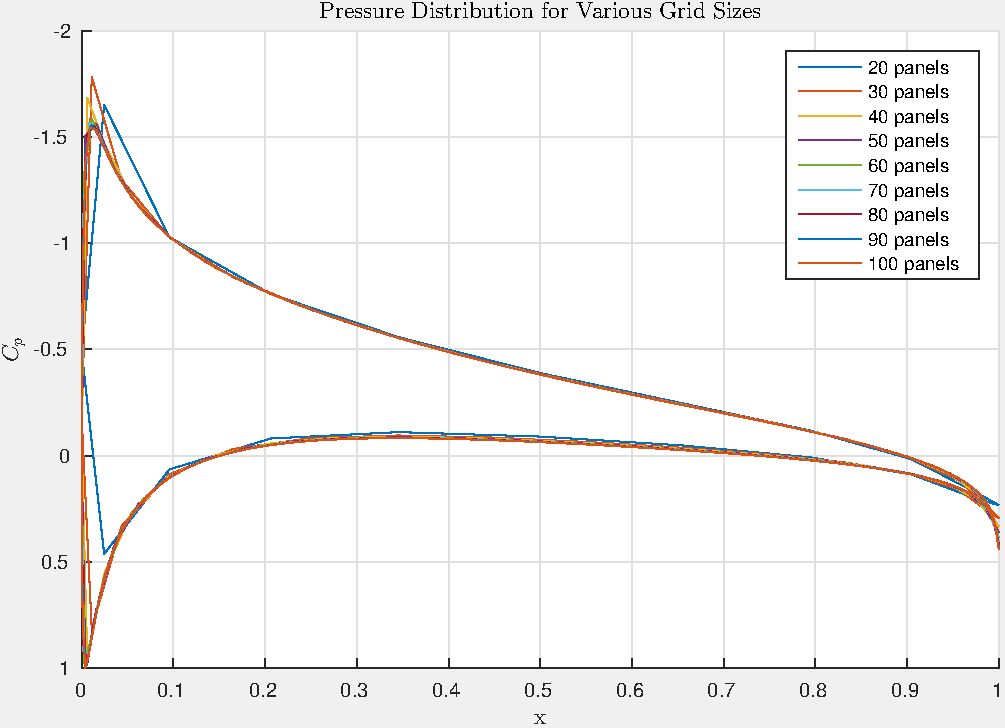
\includegraphics[width = 0.95\textwidth]{./figures/q1pressure.pdf}
    \caption{Pressure Distribution NACA0012, $Re = 1\textsc{e}06$, $\alpha = 4^{\circ}$}
    \label{fig:q1p}
\end{figure}

The pressure distribution for various number of panels is shown in Figure \ref{fig:q1p}.
As the number of panels increase, the pressure distribution converges to a smoother shape.
It is possible to visually differentiate the pressure distribution of 20, 30 and 40 panels from the other results.

The lift and drag coefficients are compiled in Table \ref{tab1}.
Their convergence are graphically shown in Figure \ref{fig:q1l} and \ref{fig:q1d}.
As the number of panels increases, the lift and drag coefficients also converge.
For lower numbers of panels, the drag coefficient is higher than its converged value and the lift coefficient is lower than its converged value.
Since less panels entails a bigger grid spacing, the truncation error is higher for coarser grids.
Numerical dissipation has stronger effects for coarse grids, resulting in weaker performances of the airfoil.

From Figure \ref{fig:q1l} and \ref{fig:q1d}, 30-40 panels seem to be sufficient to get a reasonably accurate lift coefficient, while 50 panels are required to get an accurate drag coefficient.

\begin{table}[!h]
\centering
\begin{tabular}{ccc} \toprule
    {Number of Panels} & {$C_L$} & {$C_D$} \\ \midrule
    {20} & 0.4488  & 0.0093\\
    {30} & 0.4673  & 0.0095\\
    {40} & 0.4724  & 0.0095\\
    {50} & 0.4746  & 0.0084\\
    {60} & 0.4759  & 0.0083\\
    {70} & 0.4768  & 0.0083\\
    {80} & 0.4774  & 0.0082\\
    {90} & 0.4778  & 0.0083\\
    {100} & 0.4782  & 0.0082 \\
\bottomrule
\end{tabular}
\caption{Lift and Drag Coeffcients for NACA0012, $Re = 1\textsc{e}06$, $\alpha = 4^{\circ}$}
\label{tab1}
\end{table}

\begin{figure}[!h]
    \centering
    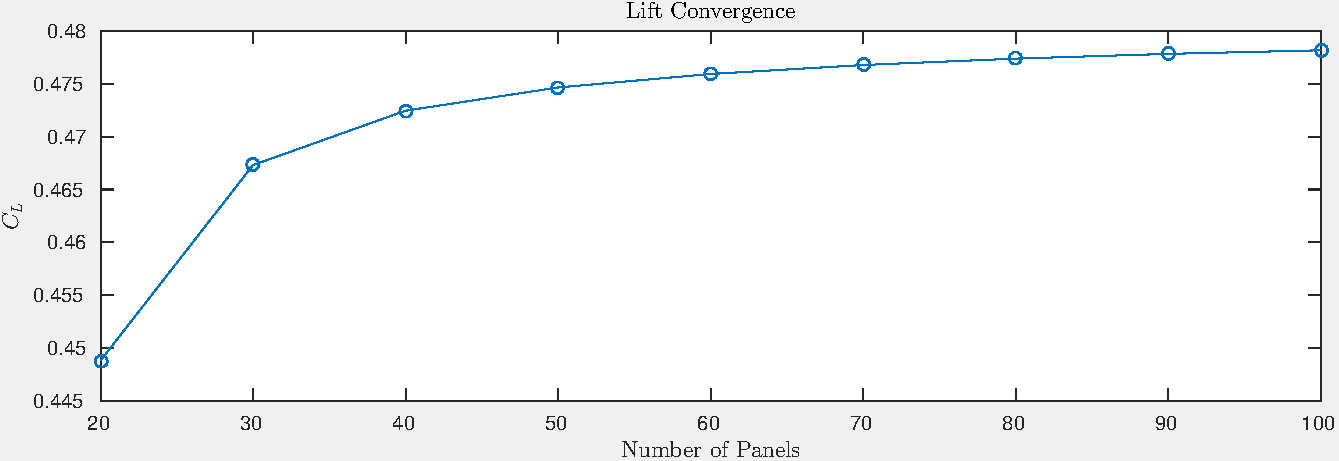
\includegraphics[width = 0.95\textwidth]{./figures/q1lift.pdf}
    \caption{Lift Grid Study}
    \label{fig:q1l}
\end{figure}

\begin{figure}[!h]
    \centering
    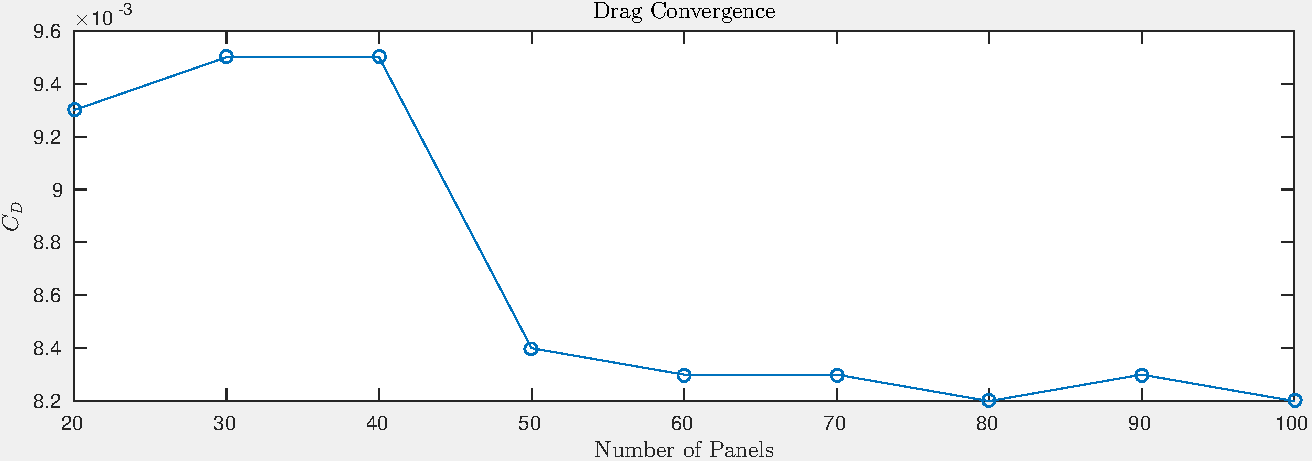
\includegraphics[width = 0.95\textwidth]{./figures/q1drag.pdf}
    \caption{Drag Grid Study}
    \label{fig:q1d}
\end{figure}

\section*{Question 2: Pressure Validation}

\begin{figure}[!h]
    \centering
    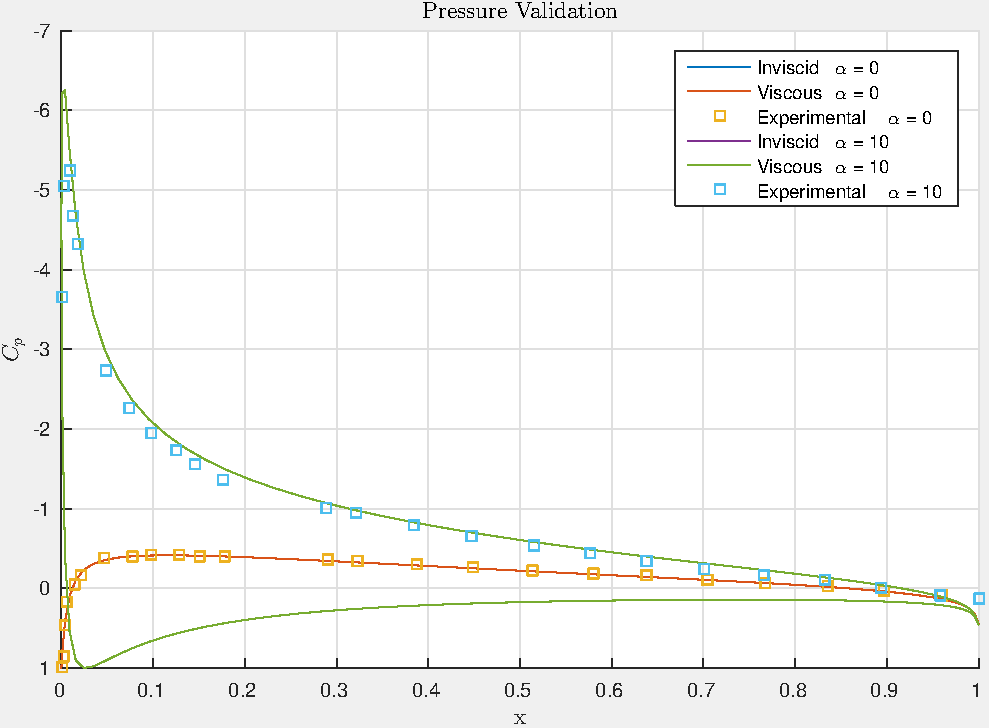
\includegraphics[width = 0.95\textwidth]{./figures/q2pressure.pdf}
    \caption{Drag Grid Study}
    \label{fig:q2}
\end{figure}

\section*{Question 3: Angle of Attack Study}

\begin{figure}[!h]
    \centering
    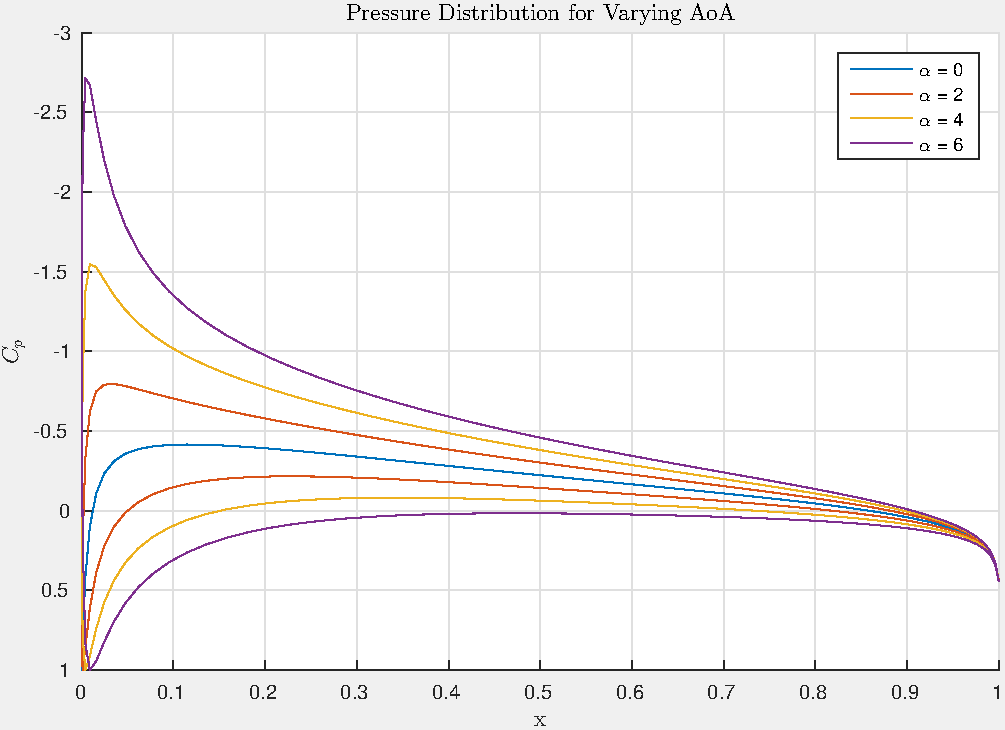
\includegraphics[width = 0.95\textwidth]{./figures/q3pressure.pdf}
    \caption{Pressure Distribution of NACA0012}
    \label{fig:q3p}
\end{figure}

\begin{figure}[!h]
    \centering
    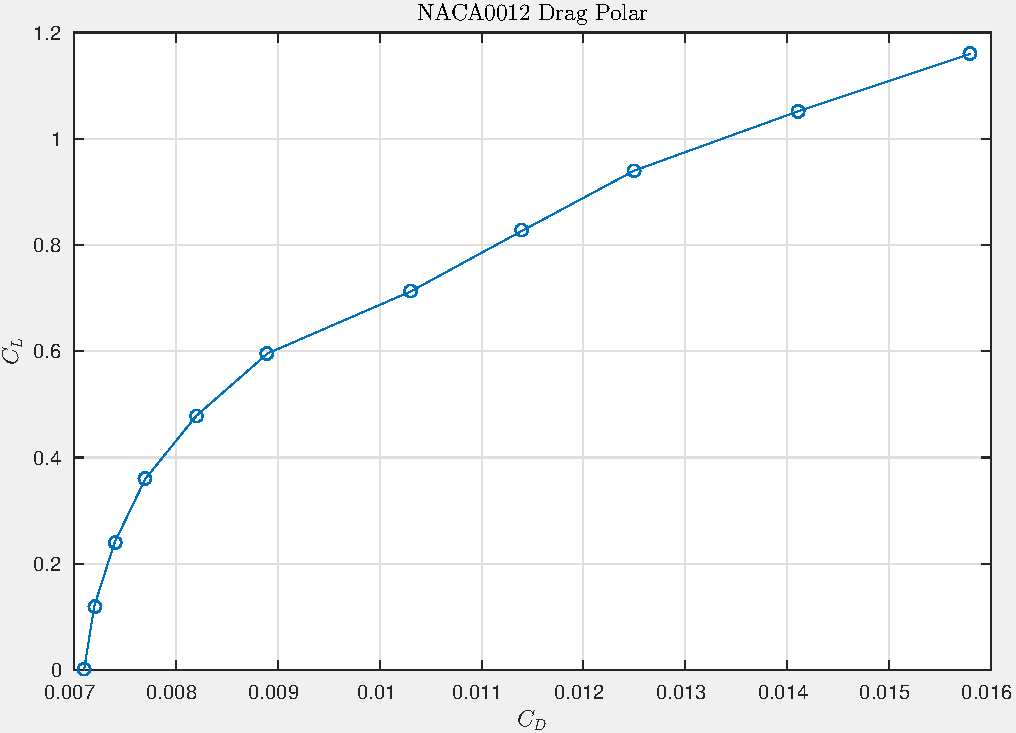
\includegraphics[width = 0.95\textwidth]{./figures/q3dp.pdf}
    \caption{Drag Polar of NACA0012}
    \label{fig:q3dp}
\end{figure}

\section*{Question 4}

\begin{figure}[!h]
    \centering
    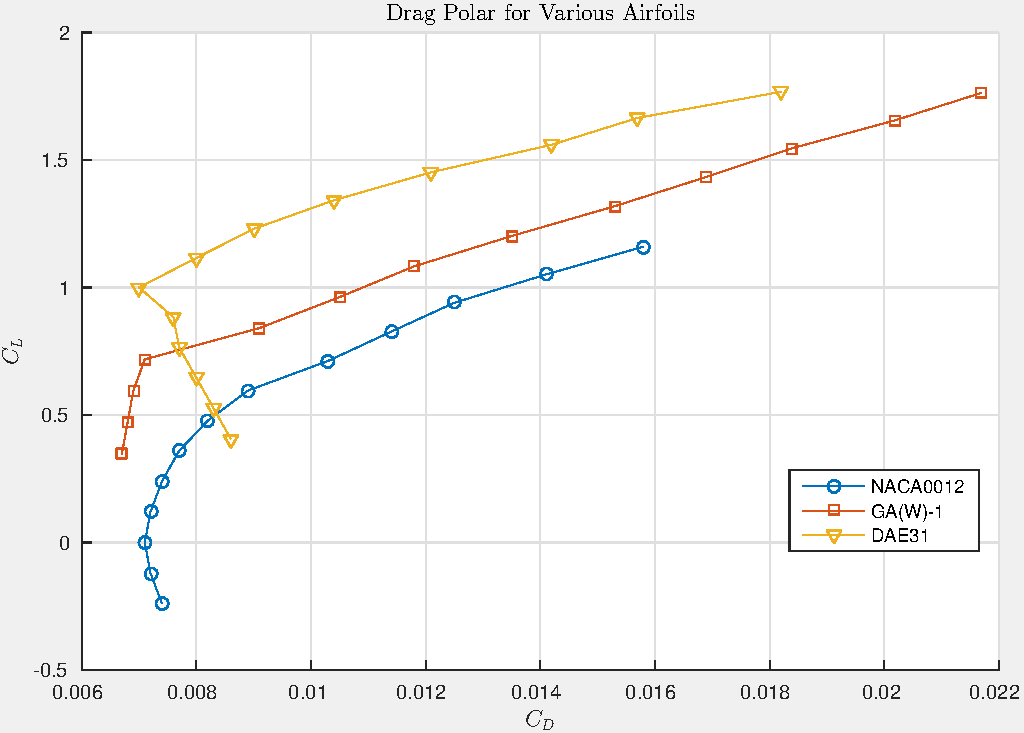
\includegraphics[width = 0.95\textwidth]{./figures/q4dp.pdf}
    \caption{Drag Polar of Various Airfoils}
    \label{fig:q4a}
\end{figure}

\begin{figure}[!h]
    \centering
    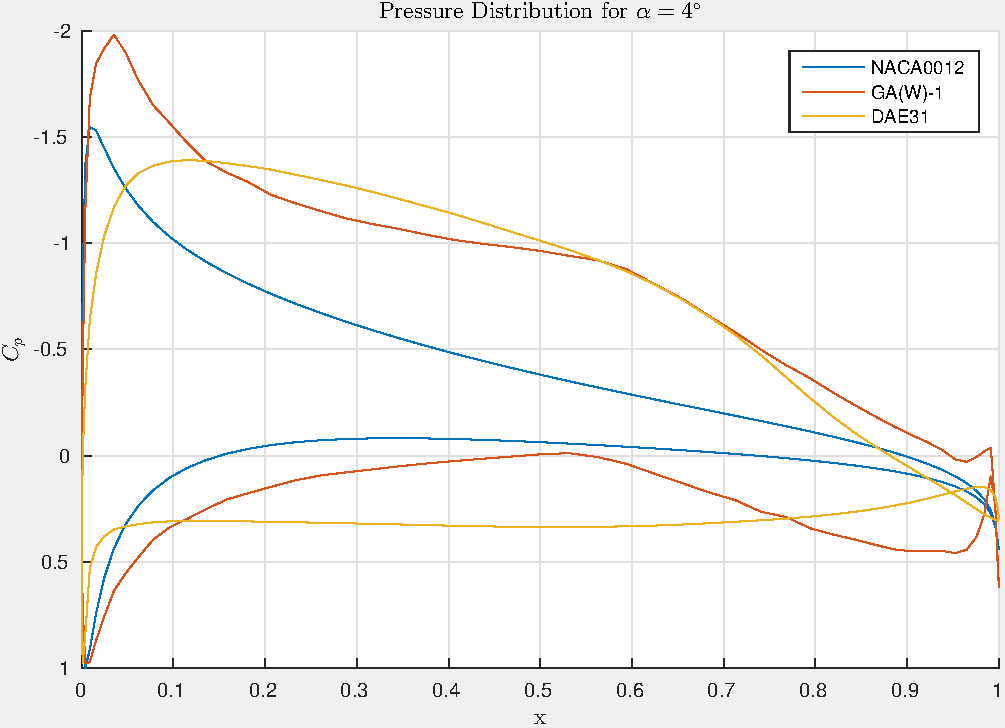
\includegraphics[width = 0.95\textwidth]{./figures/q4pressure.pdf}
    \caption{Pressure Distribution at $\alpha = 4^\circ$}
    \label{fig:q4c}
\end{figure}

\begin{figure}[!h]
    \centering
    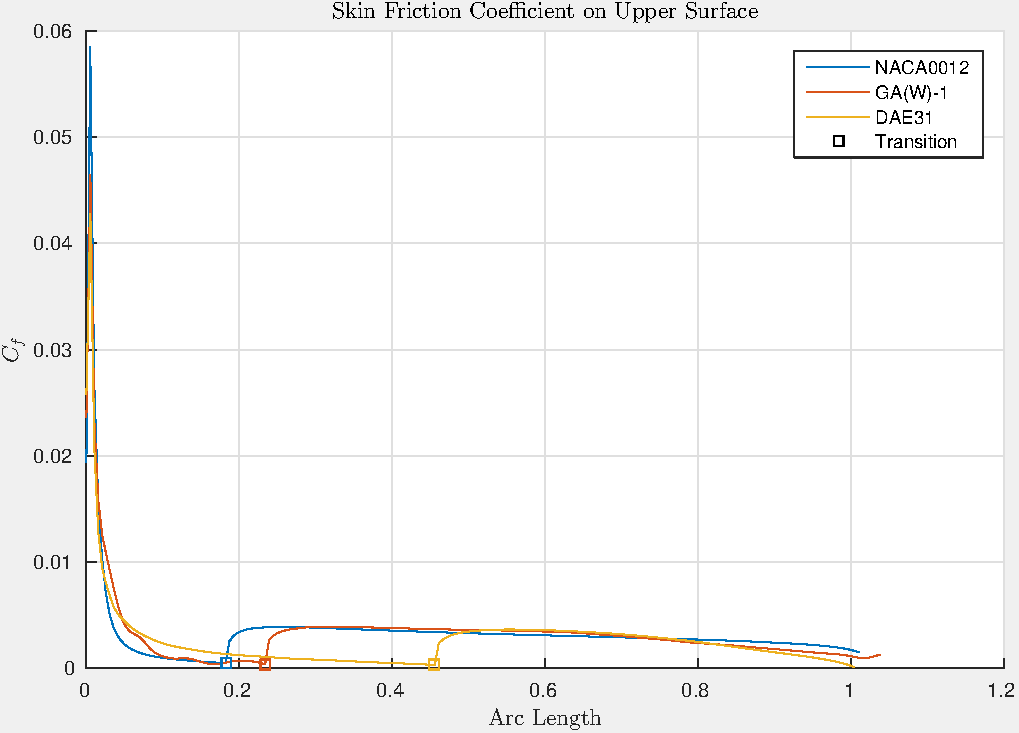
\includegraphics[width = 0.95\textwidth]{./figures/q4uppercf.pdf}
    \caption{Skin Friction Coefficient on Upper Surface at $\alpha = 4^\circ$}
    \label{fig:q4dupper}
\end{figure}

\begin{figure}[!h]
    \centering
    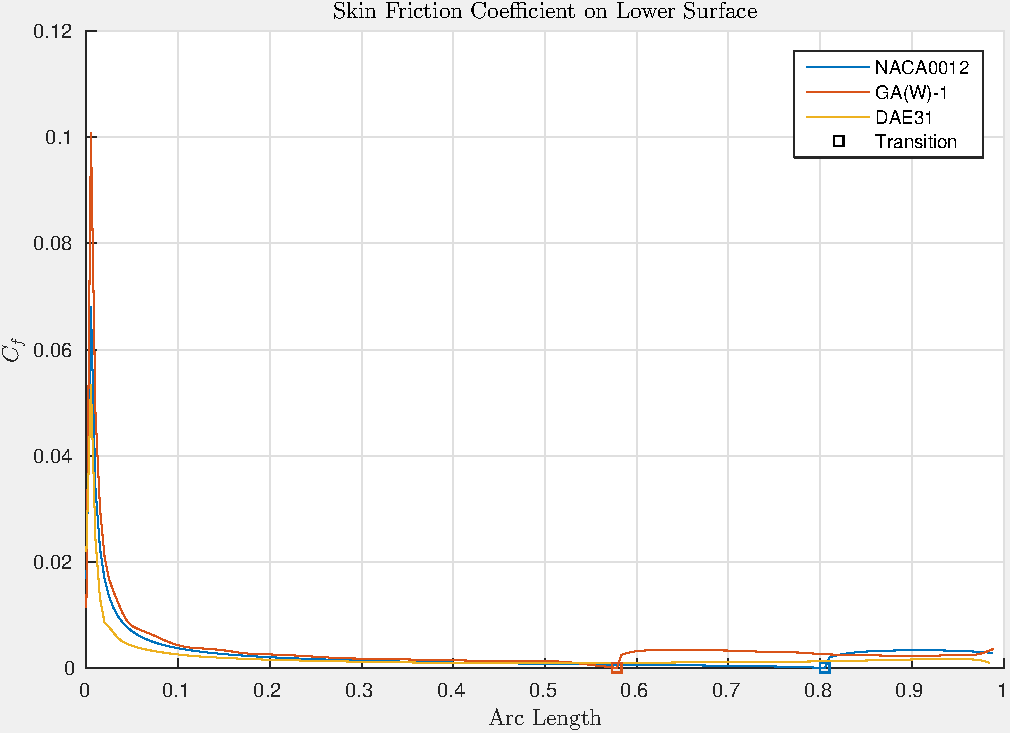
\includegraphics[width = 0.95\textwidth]{./figures/q4lowercf.pdf}
    \caption{Skin Friction Coefficient on Lower Surface at $\alpha = 4^\circ$}
    \label{fig:q4dlower}
\end{figure}

\section*{Codes}

Code has been written in FORTRAN. Default arithmetic operations are in double precision and optimization level -O3 unless specified otherwise.

All codes are available on my GitHub:

\url{https://github.com/dougshidong/mech539/tree/master/a2}

\end{document}
